\documentclass[12pt]{article}

\usepackage[symbol,perpage]{footmisc} %this is for dagger footnotes

\input quiz-setup
\newcommand{\version}{} 
\newcommand{\xzero}{}
\newcommand{\xone}{}
\newcommand{\xtwo}{}
\newcommand{\xthree}{}
\newcommand{\xfour}{}
\newcommand{\xfive}{}
\newcommand{\vecb}[1]{\mathbf{#1}}

\newcommand{\ExamName}{Quiz \#5\version}
% \newcommand{\CourseName}{Math 34A}
% \renewcommand{\Quarter}{Spring 2017}

%these are for dagger footnotes
\DefineFNsymbols*{daggorath}{{$\dagger$}{$\ddagger$}{$\dagger\dagger$}{$\ddagger\ddagger$}}
\setfnsymbol{daggorath}
\renewcommand{\thefootnote}{\fnsymbol{footnote}}
%\end dagger footnotes stuff




\begin{document}
%%
%% Version A:
\renewcommand{\version}{}
\renewcommand{\xzero}{0.0}
\renewcommand{\xone}{1.3}
\renewcommand{\xtwo}{2.9}
\renewcommand{\xthree}{4.1}
\renewcommand{\xfour}{5.3}
\renewcommand{\xfive}{6.5}
% 
\begin{minipage}{0.25\linewidth}
  \CourseName\ \Quarter \\
  \ExamName \\[1em]
  \textbf{No calculators}\\[2em]
\end{minipage}
\hfill
\begin{minipage}[t]{0.4\linewidth}
  
\begin{tikzpicture}[x=26mm,y=16mm]
    \draw[thick,black] (0,0) rectangle (3,1);
    \node[\faintcolor,right] at (0,0.2) {\large\textsf{PRINT NAME}};
  \end{tikzpicture}
\end{minipage}
\hfill
\begin{minipage}{0.25\linewidth}
  \vspace*{-3.25em}
  \ \hfill
  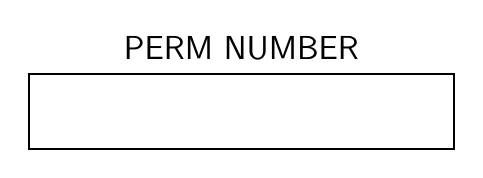
\begin{tikzpicture}[x=36mm,y=16mm]
    \node[\faintcolor] at (0.75,0.8) {\large\textsf{PERM NUMBER}};
    \draw[thick,black] (0,0) rectangle (1.5,0.6);
  \end{tikzpicture}
\end{minipage}
% \medskip
\vspace*{-0.25in}

%Put your answer in the 
%\begin{tikzpicture}[x=10mm,y=10mm,baseline=3mm] 
%  \draw[thick,black] (0,0) rectangle (3,1);
%  \node[\faintcolor] at (1.5,0.4) {\Huge\textsf{box}};
%\end{tikzpicture}
%provided.
\hfill
\begin{minipage}{0.5\linewidth}
\begin{center}

  \textbf{TA:}\ 
  \parbox[t]{0.7in}{%
    \checkbox\ \TAOne \\
    \checkbox\ \TATwo 
  }
  %\parbox[t]{0.7in}{%
  %  \checkbox\ \TAThree\\
  %  \ \ \ 
  %}
  % \ 
  % \parbox[t]{4in}{%
  % \textbf{Section Time:}
  \hfill%\hspace*{0.25in}
  % \ 
  % \parbox[t]{4in}{%
  % \textbf{Section Time:}
  \textbf{Time:}
  \parbox[t]{0.55in}{%
    \checkbox\ 4:30 \\
    \checkbox\ 5:30
  }
  \quad
  \parbox[t]{0.55in}{%
    \checkbox\ 6:30 \\
    \checkbox\ 7:30 
  }
  % }
%  \textbf{TA:}\ 
%  \parbox[t]{0.95in}{%
%    \checkbox\ \TAOne
%  }
%  \parbox[t]{0.95in}{%
%    \checkbox\ \TATwo\\
%  }
%%  \parbox[t]{0.95in}{%
%%    \checkbox\ \TAThree
%%  }
%  \hspace*{0.5in} 
%  \parbox[t]{3in}{%
%    \textbf{Section Time:}
%    \parbox[t]{0.75in}{%
%      \checkbox\ 4:30 \\
%      \checkbox\ 5:30
%    }
%    \parbox[t]{0.75in}{%
%      \checkbox\ 6:30 \\
%      \checkbox\ 7:30
%    }
%  }
\end{center}

\end{minipage}
\noindent\hspace*{-2em}\rule{\textwidth+4em}{1pt}%

\mbox{}

%\textbf{Today we will be working in groups of 3.} Discuss the following questions about exact equations with your group, and write down the answers your group comes up with. You can each write the same things, but \textbf{everyone in the group must turn in their own quiz.}



\begin{enumerate}
  \setcounter{problemnumber}{0}
\Problem \mbox{}
\begin{enumerate}
\item Consider the system of equations 
$$\vecb{x}'=\left( 
\begin{matrix}
0 & 1 & 1 \\
1 & 0 & 1 \\
1 & 1 & 0 \\
\end{matrix}
\right)\vecb{x}.$$ 
Two solutions to this system are 
$\left( 
\begin{smallmatrix} 
1  \\
1  \\
1  \\
\end{smallmatrix}
\right)e^{2t}$ 
and 
$\left( 
\begin{smallmatrix} 
1 \\
0 \\
-1 \\
\end{smallmatrix}
\right)e^{-t}$, and they are a linearly independent set\footnote{If you had to, how would you check this? [This isn't part of the question, but good to think about] }. However, without doing any computations, it can be seen that they are \emph{not} a fundamental set. Why not? [How do you know?]
\vfill

\item What do we mean when we say that a fundamental solution set \emph{spans} the set of all solutions?
\vfill

\end{enumerate}

\pagebreak
\Problem Write 3 true/false or short answer questions that you would put on the final exam if you were teaching this class. Give a key, explain the answers, then explain why you chose these particular questions and what you hope they will assess. \textbf{Each member should be writing 3 different questions from the rest of your group.} 

You will only receive credit for this problem if your questions illustrate a variety of ideas from this course, show creativity and thoughtfulness, and are conceptual questions (no ``solve this DE" or other purely computational questions). 

	\begin{enumerate}
	\item Question: \vspace*{12pt}
	
	Answer and explanation: \vfill
	
	In your role as "the teacher", why do you think this is a good exam question? What does this assess? \vfill
	
	\item Question: \vspace*{12pt}
	
	Answer and explanation: \vfill
	
	In your role as "the teacher", why do you think this is a good exam question? What does this assess? \vfill
	
	\item Question: \vspace*{12pt}
	
	Answer and explanation: \vfill
	
	In your role as "the teacher", why do you think this is a good exam question? What does this assess? \vfill
	
	\end{enumerate}

\end{enumerate}





\end{document}
